%\VignetteIndexEntry{User guide to nhm}
%\VignetteEngine{R.rsp::tex}
\documentclass{article}

%% Need to modify Sweave.sty to pass pdftex option to graphicx.
%\usepackage{Sweave-local}
\usepackage{graphics}
\RequirePackage[T1]{fontenc}
%%Check if we are compiling under latex or pdflatex
\ifx\pdftexversion\undefined
  \RequirePackage[dvips]{graphicx}
\else
  \RequirePackage[pdftex]{graphicx}
  \RequirePackage{epstopdf}
\fi
\RequirePackage{ae,fancyvrb}
\IfFileExists{upquote.sty}{\RequirePackage{upquote}}{}
\setkeys{Gin}{width=0.8\textwidth}
\newenvironment{Schunk}{}{}

\usepackage{amsmath,amsfonts,mathtools, bm, authblk}
%\usepackage[nolists]{endfloat}
\usepackage[usenames]{color}
\usepackage{subfig}
\usepackage[countmax]{subfloat}
\usepackage{rotating}
\newcommand{\prob}{\mathbb{P}}
\newcommand{\expec}{\mathbb{E}}
\newcommand{\indic}{\mathbf{1}}
\renewcommand{\baselinestretch}{1.75}
\renewcommand{\thefootnote}{\fnsymbol{footnote}}
\numberwithin{equation}{section}
\usepackage{multirow}
\usepackage{fancyvrb}

\usepackage{times}
\usepackage{url}
\addtolength{\textwidth}{2cm}

\fvset{formatcom=\singlespacing}

\DefineVerbatimEnvironment
{verbatim}{Verbatim}
{formatcom=\color{blue}, frame=none, samepage=true, baselinestretch=1.2}
\DefineVerbatimEnvironment
{verbout}{Verbatim}
{formatcom=\color{red}, frame=none, samepage=true, baselinestretch=1.2}


\setlength{\textheight}{9in} \setlength{\footskip}{0.3in}
\setlength{\topmargin}{-0.55in} \setlength{\headsep}{0.3in}
\setlength{\headheight}{0.25in} \setlength{\oddsidemargin}{0in}
\setlength{\evensidemargin}{0in} \setlength{\textwidth}{6.5in}
\setlength{\marginparsep}{0in} \setlength{\marginparwidth}{0in}
\setlength{\footskip}{1in}
\setlength{\parindent}{0cm}

\newcommand{\nc}{\newcommand}
\nc{\black}{\color{black}}
\nc{\blue}{\color{blue}}
\nc{\red}{\color{red}}

\begin{document}

\title{Non-homogeneous Markov and misclassification hidden Markov multi-state modelling in R}

\author{Andrew C. Titman}

\affil{\small School of Mathematical Sciences, Lancaster University, UK}

\maketitle

\abstract{Multi-state models are a useful approach for modelling event history data in which an individual makes transitions between a series of states over time. A Markov assumption is often made in such models and for intermittently observed data the models are usually parametric. 

The {\it nhm} package allows non-homogeneous Markov models with smoothly changing transition intensities to be fitted to intermittently observed data through direct numerical solution of the differential equations defining the transition probabilities. Misclassification type hidden Markov models with non-homogeneous transition intensities can also be fitted. The package permits models with log-linear time trends (Gompertz type intensities) to be fitted, Weibull intensities or B-spline intensity functions to be specified directly. In addition, users may also supply their own function for the generator function of transition intensities and its derivatives to allow bespoke models to be fitted.

This manual provides a brief overview of the underlying theory behind non-homogeneous Markov and misclassification hidden Markov models and also gives a tutorial on the typical use of {\it nhm}.
}

\section{Introduction}

%Some general bunff on multi-state Markov models

The likelihood for Markov models on intermittently observed data requires computation of the transition probabilities, which are the solution of the Kolmogorov Forward Equations (KFE) a system of ordinary differential equations defined by the transition intensities \cite{coxmiller}. For time homogeneous models where the intensities are constant, the KFE define a linear system of equations and hence the transition probabilities can be calculated by computing a matrix exponential. Moreover, the transition probabilities for models with piecewise constant intensities can also be found in matrix analytic form by computing matrix exponentials with respect to each time period in which the intensities are constant and combining them using the Chapman-Kolmogorov equations. Models using these matrix analytic formulations can be fitted efficiently using the {\it msm} package \cite{jackson}. 

However, the assumption of time homogeneity is often not plausible and models with piecewise constant intensities are potentially sensitive to the choice of cut points.  

%Link to msm etc.
%Something about time transformation


\section{Underlying methods}

The underlying methods implemented by the package overlap heavily with those of the {\it msm} package \cite{jackson} and the reader is encouraged to consult the {\it msm} package manual and references therein for a basic introduction to intermittently observed time homogeneous multi-state models. See in particular, Kalbfleisch and Lawless (1985) \cite{kalbfleisch} and Jackson {\it et al} (2003) \cite{jackson2003} for the seminal papers for Markov and misclassification-type Markov models, respectively.

The key extension that {\it nhm} aims to accommodate is the fitting of models where the transition intensities may be smooth functions of time.

The likelihood for an individual observed in states $x_0, x_1, \ldots, x_m$ at times $t_0, t_1, \ldots, t_m$ can be expressed as

$$L(\bm\theta) = \prod_{j=1}^{m} \mathbb{P}(X(t_j) = x_j | X(t_{j-1}) = x_{j-1} ; \bm\theta) = \prod_{j=1}^{m} p_{x_{j-1}x_j}(t_{j-1},t_j ; \bm\theta)$$
Let $\mathbf{P}(t_0, t ; \bm\theta)$ be the matrix of transition probabilities such that $\{\mathbf{P}(t_0, t)\}_{rs} = p_{rs}(t_0,t ; \bm\theta)$ then for a general non-homogeneous Markov model, these transition probabilities satisfy the initial value problem

$$\frac{d\mathbf{P}(t_0, t ; \bm\theta)}{dt} = \mathbf{P}(t_0, t ; \bm\theta)\mathbf{Q}(t ; \bm\theta), ~~ \mathbf{P}(t_0, t_0 ;\bm\theta) = \mathbf{I}$$
where $\mathbf{Q}(t ; \bm\theta)$ is the generator matrix of transition intensities. Following the approach proposed in Titman (2011), {\it nhm} uses direct numerical solution of this system of differential equations to compute the likelihood. For additional efficiency in optmization, Titman (2011) proposed to solve the extended system of differential equations, incorporating the systems of equations defining the derivatives with respect to the parameter vector $\bm\theta$:
$$\frac{d\mathbf{P}'(t_0, t ; \bm\theta)}{dt} = \mathbf{P}'(t_0, t ; \bm\theta)\mathbf{Q}(t ; \bm\theta) + \mathbf{P}(t_0, t ; \bm\theta)\mathbf{Q}'(t ; \bm\theta), ~~ \mathbf{P}'(t_0, t_0 ;\bm\theta) = \mathbf{0}$$
where $$\mathbf{P}'(t_0, t_0 ;\bm\theta) = \frac{\partial \mathbf{P}(t_0, t ; \bm\theta)}{\partial \bm\theta} ~~ \mbox{and} ~~ \mathbf{Q}'(t ; \bm\theta) = \frac{\partial \mathbf{Q}(t ; \bm\theta)}{\partial \bm\theta},$$
so that the first derivatives of the likelihood can be calculated.

The differential equations are solved by using the LSODA routine \cite{lsoda} of the deSolve package \cite{deSolve}, which automatically selects appropriate methods to allow for {\it stiff} differential equations, if necessary.

\subsection{Misclassification type hidden Markov models}

For misclassification type hidden Markov models, forward recursion is used to compute the likelihood contribution for an individual. 

Let $e_{rs} = P(O_j = s | X_j = r)$ be the $(r,s)$ entry of the misclassification matrix. Then for a subject with observed states $O_1,\ldots,O_m$ at times $t_1,\ldots,t_m$, forward weights are defined as $\alpha_{k}(j)$ for observation number $k=1,\ldots,m$ and state $j=1,\ldots,R$, where
\begin{displaymath}\alpha_{1}(j) = \prob(O_{1}, X_{1}=j) = \pi_{0j}e_{j,O_{1}},\end{displaymath}
where $\pi_{0j}$ is the $j$th entry of $\mathbf{\pi_{0}}$, and subsequent forward weights are calculated recursively:
\begin{displaymath}\alpha_{k}(j) = \prob(O_{1},\ldots,O_{k}, X_{k}=j) = \sum_{i=1}^{R} \alpha_{k-1}(i)e_{j,O_{k}}p_{ij}(t_{k-1},t_{k} ; \bm\theta).\end{displaymath}
Then the likelihood for that subject is given by
\begin{displaymath}\prob(O_{1},\ldots,O_{m}) = \sum_{i=1}^{R} \alpha_{m}(i).\end{displaymath}

To compute the first derivatives, an extended forward recursion is used as proposed by Lystig and Hughes (2002) \cite{lystig} in the context of discrete time hidden Markov models. 

If we further define
\begin{displaymath}\phi_{k}(\theta_{u},j) = \frac{\partial \alpha_{k}(j)}{\partial \theta_{u}} = \frac{\partial}{\partial \theta_{u}} \prob(O_1,\ldots,O_k,X_k = j)\end{displaymath}
then this allows $\phi_{k}(\theta_{u},j)$ to be calculated recursively as
\begin{equation}
\begin{split}
\phi_{k}(\theta_{u},j) = \sum_{i=1}^{R} \left( \phi_{k-1}(\theta_{u},i)e_{jO_{k}}p_{ij}(t_{k-1},t_{k} ; \bm\theta) + \phantom{\frac{~}{~}} ~~~~~~~~ \right. \\ \left. ~~~~~~~~~~~~~ \alpha_{k-1}(i)\frac{\partial e_{j,O_{k}}}{\partial \theta_{u}} + \alpha_{k-1}(i)e_{j,O_{k}}\frac{\partial p_{ij}(t_{k-1},t_{k};\bm\theta)}{\partial \theta_{u}} \right).
\end{split}\end{equation}
Then the first derivative of the likelihood for the subject is given as
\begin{displaymath}\frac{\partial \prob(O_1,\ldots,O_{m})}{\partial \theta_u} = \sum_{i=1}^{R} \phi_{m}(\theta_u,i).\end{displaymath}


\section{Model specification: {\it model.nhm}}
\label{model_spec}

The purpose of the function \verb!model.nhm! is to define model objects which may then be used in the main function, \verb!nhm!. \verb!model.nhm! puts the supplied data into a standardized format, builds functions for computing the generator or intensity matrix and its derivatives and, in the case of misclassification models, also creates functions for computing the misclassification probabilities and initial state occupation probabilities. 

\subsection{Identification of key variables}

The \verb!formula! argument follows the same syntax as used in the {\bf msm} package. A formula should be provided where the left hand side identifies the state variable and the right hand side identifies the time variable. For example \verb!formula = state ~ years! implies that the observed states are stored in a column named \verb!state! while the corresponding observation times are in a column \verb!years!. 

The \verb!data! argument identifies the name of the data frame in which the data are stored. Note that this cannot be omitted. The \verb!subject! argument identifies the name of the subject identifier variable within the data frame. The \verb!covariates! argument should be a character vector giving the names of the covariates that are used in the model. These variables should be columns within the \verb!data! data frame. Note that these covariates could be used in either the model for the transition intensities or, in the case of misclassification models, for covariate effects on the misclassification probabilities or initial state probabilities.

\subsection{Generator matrix {\it type}}

The \verb!type! argument specifies the type of non-homogeneous model for the generator or intensity matrix of the Markov process. The possible values are \verb!'gompertz'!, \verb!'weibull'!, \verb!'bspline'! and \verb!'bespoke'!.

\subsubsection*{Gompertz type}

A \verb!'gompertz'! type model leads to models where some or all of the intensities are of the form

$$q_{rs}(t ; \mathbf{z}) = \exp( \theta_{rs} + \beta_{rs}(t - \bar{t}) + \bm\gamma_{rs}^{'}\mathbf{z})$$

where $\beta_{rs}$ defines a log-linear trend in intensity with respect to time, with the model reducing to time homogeneity if $\beta_{rs}=0$. Here, $\bar{t}$ is an optional centring term which reparametrizes $\theta_{rs}$ to refer to the baseline intensity value at $t = \bar{t}$ rather than 0. Such centring can be specified using the optional argument \verb!centre_time! and usually helps with convergence of the maximum likelihood algorithm.

\subsubsection*{Weibull type}

A \verb!'weibull'! type model leads to models where some or all of the intensities are of the form

$$q_{rs}(t ; \mathbf{z}) = \lambda_{rs} \alpha_{rs} (\lambda_{rs} t)^{\alpha_{rs} - 1} \exp(\bm\gamma_{rs}^{'}\mathbf{z})$$
where $\alpha_{rs} >0$ is the shape parameter, $\lambda_{rs} > 0$ the rate parameter. A time homogeneous model arises with $\alpha_{rs} = 1$. 
In {\it nhm}, in order to allow the likelihood to be maximized via unconstrained optimization, the model is parametrized in terms of the log-shape, $a_{rs}$, and log-rate, $\theta_{rs}$,

$$q_{rs}(t ; \mathbf{z}) = \exp\left\{ \theta_{rs} \exp(a_{rs}) + (\exp(a_{rs}) - 1)\log t  +\bm\gamma_{rs}^{'}\mathbf{z}\right\}.$$

\subsubsection*{B-spline type}

A \verb!'bspline'! type model leads to models where some or all of the intensities are of the form

$$q_{rs}(t ; \mathbf{z}) = \exp\left\{ \theta_{rs} + \bm\nu_{rs}^{'}\mathbf{B}(t) +\bm\gamma_{rs}^{'}\mathbf{z}\right\}$$

where $\mathbf{B}(t)$ is the vector of B-spline basis functions at time $t$ for a B-spline of a certain order with certain knot points, implying the overall effect of time is represented by a spline function that is a smooth piecewise polynomial. Note that this specification differs slightly from that used in Titman (2011).

The knot points for the spline are specified using the argument \verb!splinelist!. This should be a list of length equal to the number of distinct spline effects in the model, of vectors which specify the location of the knots of the spline (including the boundary knots). By default the splines are of degree 3, but this can be modified by using the \verb!degrees! argument. 

\subsubsection*{Bespoke type}

If a non-homogeneous model not built into the package is desired, the \verb!'bespoke'! type can be specified. To fit a bespoke model, it is necessary to also provide a function that computes the generator (transition intensity) matrix and its derivatives at a given time \verb!t!, covariate vector \verb!z! and vector of model parameters \verb!x!. It should output a list containing a matrix \verb!q! and an array \verb!qp!. The matrix \verb!q! should be the $R \times R$ matrix $\mathbf{Q}(t; z, \bm\theta)$ whose $(r,s)$ entry is $q_{rs}(t; z, \bm\theta)$ for $r \neq s$ and $-\sum_{k} q_{rk}(t;z,\bm\theta)$ for $r = s$. The array \verb!qp! should be the $R \times R \times n_p$ array of first derivatives
${d\mathbf{Q}(t ; z, \bm\theta)}/{d\bm\theta}$, where $n_p$ is the number of parameters in the model for the generator matrix.

Although not required, it is desirable to provide an attribute to the function named \verb!npar! that stores $n_p$. In addition, parameter names (for use in \verb!print!) can be supplied in an attribute \verb!parnames!. The attribute should be a character string of length $n_p$. The created function should be supplied as the argument \verb!intens!. 

Note that for large models or datasets or if the same model will be fitted many times, it is general advantageous to hard code an \verb!intens! function even if the model is one of the pre-specified types. The speed gain varies, but may be biggest for models with a large(r) number of covariates that only affect a small number of transitions.

%Provide an example


\subsection{{\it trans} argument}

The number of states in the model and the set of admissible transitions is specified using the \verb!trans! argument. \verb!trans! should be an $R \times R$ matrix. The $(r,s)$ entry should be 0 if the $r \rightarrow s$ transition is inadmissible. The admissible transitions should be numbered consecutively from 1. If the same number is given to two or more distinct transitions, e.g. $(r,s)$ and $(r',s')$, then this implies $\theta_{rs} = \theta_{r's'}$, i.e. the baseline parameters for each transition are constrained to be equal.

The diagonal of the matrix will be ignored, but a warning is given if it contains entries other than 0.

For \verb!bespoke! type models, \verb!trans! is only used to specify the number of states in the model, i.e. it can be an $R \times R$ matrix of zeroes.

\subsection{{\it nonh} argument}

The \verb!nonh! argument specifies which transition intensities are non-homogeneous with respect to time. The same principles as the verb!trans! argument holds. \verb!trans! should be an $R \times R$ matrix. If the $(r,s)$ entry is 0 it implies either the transition is inadmissible or it is time homogeneous. The non-homogeneous transitions should be numbered consecutively from 1. If the same number is given to two or more transitions then it is assumed they have the same time trend parameter(s). For instance for a Weibull type model it would imply that $\alpha_{rs} = \alpha_{r's'}$.

\subsection{{\it covm} argument}

The \verb!covm! argument is used to specify which transitions are affected by which covariates. The argument can either be supplied as a named list of $R \times R$ matrices or else an $R \times R \times n_c$ array, where $n_c$ is the length of the \verb!covariates! argument. 

If a named list is supplied, the names must be present in the \verb!covariates! vector. If an array is supplied, the $(r,s, k)$ entry will relate to the effect of the $k$th covariate named in the \verb!covariates! vector on the $r \rightarrow s$ transition. The same principle used in \verb!trans! and \verb!nonh! is used for \verb!covm!. A zero entry implies no effect, otherwise effects should be numbered consecutively from 1. Assigning the same number to any two entries implies a common covariate effect. {\bf NB:} The numbering applies across the whole argument.

\subsubsection{Time dependent covariates}

Time dependent covariates may be included in the model. Time dependent covariates are assumed to be constant between observed visit times. The same data convention as the {\it msm} package is used, namely that  the transition intensities for the period $(t_i, t_{i+1})$, will be governed by the covariates measured at $t_i$. As a consequence the covariates supplied for the last follow-up time will only be used in the case of exact death times (or for covariates on misclassification probabilities). Note that a particular advantage of {\it nhm} is that deterministic time dependent covariates can be incorporated into the model without using a piecewise constant approximation. For instance, if current age is to be a covariate such that
$$\lambda_{rs}(t ; \mbox{age}(t)) = \exp(\theta_{rs} + \beta_{rs} \mbox{age}(t))$$
then this can be fitted via a ``Gompertz" model
$$\lambda_{rs}(t ; \mbox{age}(t)) = \exp(\theta_{rs} + \beta_{rs} (\mbox{age}_0 + t))$$
where $\mbox{age}_0$ is the patient's age at time 0. 
Note that the \verb!centre_time! argument can be a vector, so supplying the vector of $-\mbox{age}_0$ will allow this model to be fitted. More complicated time dependent covariates can be accommodated using a \verb!bespoke! type intensity function.

\subsection{Example: Gompertz model with covariate effects}
\label{sec:gomp_model1}

We consider a four state progressive model where the generator matrix is of the form
$$\mathbf{Q}(t; \mathbf{z}) = \begin{bmatrix} -q_{12}(t  ; \mathbf{z}) & q_{12}(t  ; \mathbf{z}) & 0 & 0 \\
0 & -q_{23}(t ; \mathbf{z}) & q_{23}(t ; \mathbf{z}) & 0 \\
0 & 0 &-q_{34}(t ; \mathbf{z}) & q_{34}(t ; \mathbf{z}) \\
0 & 0 & 0 & 0 \end{bmatrix}$$

To specify that $1 \rightarrow 2$, $2 \rightarrow 3$ and $3 \rightarrow 4$ are the only admissible transitions and that they have distinct baseline intensity parameters:
\begin{verbatim}
trans <- rbind(c(0,1,0,0),c(0,0,2,0),c(0,0,0,3),rep(0,4))
\end{verbatim}

We desire a model where all transitions have distinct time effects

\begin{verbatim}
nonh <- rbind(c(0,1,0,0),c(0,0,2,0),c(0,0,0,3),rep(0,4))
\end{verbatim}

and that each of the covariates affects the $1 \rightarrow 2$ only

\begin{verbatim}
covm <- list(
cov1 = rbind(c(0,1,0,0),rep(0,4),rep(0,4),rep(0,4)),
cov2 = rbind(c(0,2,0,0),rep(0,4),rep(0,4),rep(0,4)))
\end{verbatim}

The call to \verb!model.nhm! is then

\begin{verbatim}
gomp_model <- model.nhm(state~time, data=example_data1, subject = id, covariates=c("cov1",
"cov2"),type="gompertz",trans=trans,nonh=nonh,covm=covm)
\end{verbatim}

\subsection{Arguments for misclassification models}
\label{miscarg_sec}

The arguments \verb!emat!, \verb!ecovm!, \verb!firstobs!, \verb!initp!, \verb!initp_value! and \verb!initcovm! are specific to misclassification type hidden Markov models.

\subsubsection{Misclassification probabilities}

The general model for the misclassification probabilities is of the form

$$P(O_j = s | X_j = r, \mathbf{z}, \bm\theta) = \frac{\exp( u_{rs})}{\sum_{k} \exp(u_{rk})}$$
where $u_{rr} \equiv 0$ and $u_{rs} = \eta_{rs} + \bm\tau_{rs}^{'}\mathbf{z}.$
Hence a multinomial logistic regression model is used for each state, with correct classification taken as the baseline.

The \verb!emat! argument follows the same principles as \verb!trans! in that it should be an $R \times R$ matrix numbered consecutively from 1. Inadmissible misclassification is labelled 0, while assigning the same number to two transitions implies that $\eta_{rs} = \eta_{r's'}$.
\verb!ecovm! follows the same principles as \verb!covm! in defining the covariate effects $\bm\tau$.

\subsubsection{Initial state probabilities}
\label{initprobs}

For Markov models without misclassification, the likelihood is computed conditional on the first observed state. In contrast, for misclassification models there are several different possible ways the process could be started. The purpose of the \verb!firstobs! argument is to identify which of these possibilities applies.

\subsubsection*{The {\it firstobs} argument}

Specifying \verb!firstobs="exact"! implies that the state occupied at the first observation time was known without misclassification for all patients. This is the default if \verb!firstobs! is not specified.

Specifying \verb!firstobs="absent"! implies that no state was actually observed at the first observation time for each patient. Instead all that is assumed is the process was initiated at that time, with the state occupation probabilities at that time based on the model for initial probabilities. Note that the values of the first observations given in the \verb!state! variable in this case are effectively place-holders required only to specify the time at which the patient's process was initiated.

Specifying \verb!firstobs="misc"! implies that the state observed at the first observation time was subject to misclassification, with the distribution of true occupied states at that time based on the model for initial probabilities.

\subsubsection*{Model for initial probabilities}

If \verb!firstobs! is taken to be either \verb!'absent'! or \verb!'misc'! then a model for the state occupation probabilities at the first observation time is needed. By default, if no other arguments are specified it is  assumed that the subject  is in state 1 with probability 1. 

One can either specify a fixed vector of initial probabilities using the \verb!initial_value! argument or the initial probabilities can be allowed to follow a multinomial logistic regression model with state 1 taken as the baseline category and the parameters assumed unknown and to be estimated. In the former case \verb!initial_value! should be a numerical vector of length $R$ of non-negative values which sum to 1, corresponding to $P(X(t_0)= r), r=1, \ldots, R$. In the latter case the argument \verb!initp! should be a vector of length $R$ which identifies which states other than 1 have a non-zero probability of being occupied at the initial time. As above, the states should be numbered consecutively from 1. If the same number is assigned twice or more it implies the same baseline parameter is used. The first entry of the vector is ignored, but expected to be 0. In addition \verb!initpcovm! can be supplied to allow covariate effects on the initial probabilities. This should either be a named list of vectors of length $R$ or an $R \times n_c$ matrix.

\subsection{Further arguments}

\subsubsection{`Exact' death times}

When a multi-state model describes life history data and absorbing states correspond to death or different causes of death, it is common for the time of death to be known up to the exact day. Treating the death time as if it were a discrete event time leads to bias. To ensure the correct likelihood contribution, \verb!death = TRUE! should be specified and \verb!death.states! should be a vector identifying which of the states is subject to exact death times. Note \verb!death.states! should correspond to absorbing states within the data.

\subsubsection{Censoring}

For life history data, the end of follow-up for death may not correspond to the last observation time. For instance, the last observation of a patient may be at 5 years of follow-up, but the study ends at 7 years of follow-up. While we do not know the state occupied at 7 years, the absence of a death time can be assumed to be evidence that the patient is still alive. As such the patient's state occupied at 7 years is censored within the set of living states. 

To accommodate this situation the supplied data should include the times of end of follow up for censored individuals with a corresponding censoring code or codes. The argument \verb!censor! should be a vector of numerical censoring codes, while \verb!censor.states! should be a list of vectors specifying the corresponding sets of possible states implied by the censoring codes. For instance
\verb!censor=c(98,99)! and \verb!censor.states=list(1:2,1:3)! specifies that \verb!98! implies the individual is in either state 1 or 2, while \verb!99! implies the individual is in either state 1, 2 or 3. If  \verb!censor! is a single value then \verb!censor.states! can be specified as a vector.

For models without misclassification, censoring can only occur as the last observation in a patient's sequence. Since version 0.1.2, misclassification models can accommodate censoring at any position within a patient's sequence. Note that a model without explicit misclassification can be treated as one by supplying an \verb!emat! argument that is simply an $R \times R$ matrix of zeroes (implying the misclassification matrix is always the identity matrix).

\subsection{Output of {\it model.nhm}}

The \verb!model.nhm! function outputs an object of class \verb!nhm_model!. The print method for this object prints some basic information on the model specified; the type of model fitted, the number of unknown parameters and a table describing the individual parameters in the model. It is useful to check the output of the model specification to ensure it is as expected. It can also help when specifying initial parameter values in the \verb!nhm! function.

The table of parameters includes a `type' column. For non-bespoke generator matrix models this identifies which parameters correspond to baseline parameters (\verb!Trans! - $\theta_{rs}$), which parameters correspond to those defining non-homogeneity (\verb!Nonhom! - $\beta_{rs}$, $a_{rs}$ or $\nu_{rs}$), which to the covariate effects on the intensities (\verb!Cov! - $\bm\gamma_{rs})$, which to parameters for the misclassification model (\verb!Emat!) and which to the initial state probabilities model (\verb!Initp!). For models of bespoke type, all the parameters relating to the generator matrix are taken to be of \verb!Bespoke! parameter type.
The identification of the \verb!Nonhom! type parameters is important for the default functioning of the score test options (see Section \ref{sec:scoretest})

For the example in Section \ref{sec:gomp_model1}, the output is as follows:

\begin{verbatim}
gomp_model
\end{verbatim}
\begin{verbout}
nhm model object for a Markov model.

Model for intensities has 8 unknown parameters and is of gompertz type.
 
                    Name   Type
1             Base: 1->2  Trans
2             Base: 2->3  Trans
3             Base: 3->4  Trans
4            Trend: 1->2 Nonhom
5            Trend: 2->3 Nonhom
6            Trend: 3->4 Nonhom
7 Covariate: cov1 1 -> 2    Cov
8 Covariate: cov2 1 -> 2    Cov
\end{verbout}


\section{Model fitting: {\it nhm}}

Once a model object has been created using \verb!model.nhm! it can be passed to the main function \verb!nhm!, which allows the likelihood to be computed and maximized. 

The arguments of \verb!nhm! control the way in which the model is maximized and which model outputs are required.

The \verb!model_object! argument is for the \verb!nhm_model! object created using \verb!model.nhm!. 

\subsection{Specification of initial parameter values}

The \verb!initial! argument should correspond to the vector of initial parameter values. This should be a numeric vector of length equal to the number of unknown parameters in the model. For models without misclassification \verb!initial! can be omitted and \verb!gen_inits=TRUE! may be specified. In that case the initial parameter values are specified by calling the function \verb!crudeinits.msm! from the {\bf msm} package. Specifically initial parameters for the baseline transition intensities are found by assuming a homogeneous Markov model and that the observation times correspond to the exact transition times. Covariate effects and any non-homogeneity parameters are all set to zero. This method is not available for models with misclassification.

Note that the choice of initial parameter values can be very important to the eventual success of the optimization routine. Poor initial values may lead either to the optimization routine taking much longer to converge, or could lead to non-convergence. It can also cause problems for the computation of the transition probabilities (see [...] below).

It is best to build the model incrementally. A good starting point is usually a time homogeneous model. A time homogeneous version of the model can be fitted using {\bf msm} and those parameters can be used as starting values. Unfortunately, due to the differences in syntax and the wider range of options in {\bf msm} this process is not currently automated.


\subsection{Control options}

The \verb!nhm! function contains a \verb!control! argument. The function \verb!nhm.control! should be used to create the list of control options.

\subsubsection{Options for \it{deSolve}}

The control options \verb!tmax!, \verb!rtol!  and \verb!atol! relate to parameters to be passed to the \verb!lsoda! function within {\it deSolve}. The option \verb!tmax! determines the maximum point at which the system of differential equations should be solve, while \verb!rtol! and \verb!atol! specify the relative and absolute tolerance levels it should use.

\subsubsection{Algorithm options}
\label{alg_sec}

In general the likelihood is optimized by using Newton-type algorithms in which the parameters are updated in the form
$$\bm\theta^{(i+1)} = \bm\theta^{(i)} - \delta^{(i)} \mathbf{\tilde{H}}(\bm\theta^{(i)})^{-1}\mathbf{u}(\bm\theta^{(i)})$$ 
where $\mathbf{u}(\bm\theta) = \frac{\partial \log L(\bm\theta)}{\partial \bm\theta}$, $\mathbf{\tilde{H}}(\bm\theta^{(i)})$ is some estimate of the Hessian and $\delta^{(i)}$ is some scalar, usually in $[0,1]$, that determines the step length.

\subsubsection*{BHHH algorithm}

The default optimization method used by \verb!nhm! is the BHHH algorithm \cite{bhhh}, implemented through the \verb!maxLik! package \cite{maxLik}. The BHHH algorithm exploits the identity $\mathbb{E}(\mathbf{U}\mathbf{U}^{'}) = \mathbb{E}(\mathbf{I})$. This is a quasi-Newton algorithm in which the Hessian is approximated by $-\mathbf{J}(\bm\theta^{(i)})$ where 
$$\mathbf{J}(\bm\theta^{(i)}) = \sum_{i=1}^{N} \mathbf{u}_i(\bm\theta^{(i)}) \mathbf{u}_i(\bm\theta^{(i)})^{'}$$
where $\mathbf{u}_i(\bm\theta^{(i)}) = \frac{\partial log L_i(\bm\theta^{(i)})}{\partial \bm\theta}$ and $L_i(\bm\theta^{(i)})$ is the likelihood contribution for subject $i$. If taking $\delta^{(i)} = 1$ does not result in an improvement to the likelihood, the algorithm will repeatedly halve the step length. The degree of detail of the progress of the BHHH algorithm that is printed can be controlled using \verb!print.level! which should be an integer between 0 and 3. Further control options of the algorithm can be passed to {\it maxLik} using \verb!maxLikcontrol!.

\subsubsection*{Fisher scoring}

For models without misclassification, censoring or exact death times, a Fisher scoring algorithm can instead be used by specifying \verb!fishscore=TRUE!.  This uses minus the expected Fisher information as the estimate of the Hessian. For models that are well identified and are supplied good starting values, the Fisher scoring algorithm tends to be quicker. However, by default the algorithm is not very robust and may fail if the log-likelihood surface is quite flat or if a poor set of initial parameters is supplied. There are some additional options available to improve the robustness; \verb!linesearch! allows a line search to be performed at each iteration to find the best step length, $\delta^{(i)}$. For models that are close to non-identifiable, the algorithm can be modified so that a diagonal term is added to the expected Fisher information, i.e. $\mathbf{\tilde{H}}(\bm\theta^{(i)}) = - \left\{\mathbb{E}(\mathbf{I}(\bm\theta^{(i)})) + \lambda \mathbf{I}_p\right\}$ where $\mathbf{I}_p$ is a $p \times p$ identity matrix. This modification can be specified by setting \verb!damped=TRUE! and the damping parameter $\lambda$ can be specified using \verb!damppar!. 

By default, for either the BHHH or Fisher scoring algorithms, a finite differences estimate of the observed Fisher information, $-\frac{\partial^2 \log L}{\partial \bm\theta\partial \bm\theta^{'}}$, is computed. This requires an additional $2p$ evaluations of the likelihood gradient. While the observed information is generally considered to give more accurate standard error estimates, if \verb!obsinfo=FALSE! then \verb!nhm! will instead only provide either the expected Fisher information (in the case of the Fisher scoring algorithm) or $\mathbf{J}(\hat{\bm\theta})$ (in the case of the BHHH algorithm). 

\subsubsection*{Constrained optimization}

If the option \verb!constrained! is set to \verb!TRUE! then the NLMINB algorithm \cite{gay}, implemented via \verb!nlminb()! in the \verb!stats! package, is used for optimization. The square of the individual score contributions is supplied to the \verb!hessian! argument (rather than the exact Hessian), which leads to similar behaviour to the BHHH algorithm. However, \verb!nlminb! allows lower and upper bounds to be specified for each of the parameters to be optimized. The main practical reason to use constrained optimisation is in order to make the algorithm more robust. Particularly for datasets with long follow-up periods and/or for models with Gompertz-type (log-linear) transition intensities, unless very good starting values are supplied there is significant potential for other algorithms to propose parameter values which lead to either numerical under/overflow or a zero value for the likelihood (see also Section \ref{splits_sec}). The \verb!lower! and \verb!upper! arguments can be used to force each parameter to stay within some plausible range, where the aim is to ensure that the magnitude of the resulting transition intensities cannot get either too high or too low to lead to under/overflow problems. Potentially, this process may need to be iterative: if the algorithm still fails it may be necessary to enforce stricter limits, whilst if the algorithm converges with one of the parameters at its lower or upper boundary, it would be necessary to restart with less stringent bounds.

\subsubsection{Splits}
\label{splits_sec}

By default \verb!nhm! finds the transition probabilities by solving a single initial value problem for each unique covariate pattern. Specifically, an initial boundary problem of the form
\begin{equation}\frac{d\mathbf{P}(t_0, t ; \mathbf{z})}{dt} = \mathbf{P}(t_0,t ; \mathbf{z})\mathbf{Q}(t ;  \mathbf{z}) ~ \mbox{for}  ~ \mathbf{P}(t_0,t_0 ; \mathbf{z}) = \mathbf{I} \label{diff_eq1} \end{equation}
is solved, for all times in the set of start and end times for intervals with covariate pattern $\mathbf{z}$ and where $t_0$ is the first start time in the set.
By the identity $\mathbf{P}(t_0 , t_2; \mathbf{z}) = \mathbf{P}(t_0 , t_1; \mathbf{z})\mathbf{P}(t_1 , t_2; \mathbf{z})$ any individual transition probability can be obtained from the solutions to (\ref{diff_eq1})
$$\mathbf{P}(t_1 , t_2; \mathbf{z}) = \mathbf{P}(t_0 , t_1; \mathbf{z})^{-1}\mathbf{P}(t_0 , t_2; \mathbf{z}).$$
However, this method relies on $\mathbf{P}(t_0 , t_1; \mathbf{z})$ being invertible. The transition probability matrix may become singular if $t_0$ and $t_1$ are far apart and, for instance, the probability of remaining in a state over that time gets very close to zero. A singular matrix is most likely when poor starting values have been supplied to the optimization, but could also happen for data sets where the vast majority of individuals progress during the follow-up time.

If the algorithm fails due to a singular matrix, an error message will appear informing between which times $(t_0, t_1)$ the singularity arose. Singularities can be avoided by using the \verb!splits! option within \verb!nhm.control!. Specifically, by supplying a vector of split times, \verb!nhm! will categorize the start times into groups and solve separate initial value problems for any intervals within start times in the different groups. For instance, if a split is included at $t=5$ then $P(6,11)$ will be found by solving an initial value problem starting at the first time beyond $5$ rather than from the smallest time with that covariate pattern. Adding splits will tend to increase the computation time, but not substantially. 

The control option \verb!safe! forces the functions to always solve a new initial value problem for each unique combination of start time $t_0$ and covariate pattern. While this avoids the need to define \verb!splits!, it will typically lead to a significant increase in computation time. Note that depending on the model and starting values, the algorithm may still fail if appropriate parameter constraints have not been set (see Section \ref{alg_sec}).

\subsubsection{Coarsening covariates}

Usually, the majority of the computation time in evaluating the likelihood arises through the solution of the differential equations. The necessity to solve a separate system of equations for each covariate pattern means that models with continuous covariates can be substantially more computationally demanding.

It may be desirable for large datasets with continuous covariates to consider an approximation to the likelihood based upon coarsening the set of unique covariate values. Titman (2011) \cite{titman} proposed a simple method based on using K-means clustering to group similar values of the continuous covariates and assuming approximating transition probabilities within the same cluster by the transition probability that would arise from the mean covariate values within that cluster. While coarsening the covariates will tend to introduce some attenuation bias in the covariate effects, it may be useful either in the model building stage or in cases where the full model is computationally impractical.

\subsubsection{Parallelization}

An alternative way to speed up the computation of mdoels for data with a large number of unique covariate patterns is to exploit parallel processing. The \verb!ncores! option allows the \verb!mclapply! function in the {\bf parallel} package to allow multiple systems of ODEs to be solved simultaneously.

For models with misclassification, \verb!mclapply! is also used to simultaneously perform the forward algorithm on multiple separate individuals.

By default, if \verb!ncores!$>1$ and \verb!obsinfo=TRUE! then the package will parallelize across the complete gradient calls used to compute the observed Fisher information via finite differences. This should generally be more efficient as there should be less waiting time for all cores to complete. However, for large datasets this could cause memory issues. If \verb!parallel_hess=FALSE!, the package will instead continue to exploit parallel processing within each gradient call in the same way as during the main optimization. 

\subsection{Fixed parameters}

While \verb!model.nhm! allows parameters to be fixed to zero (e.g. no transition, no time non-homogeneity, no covariate effect etc.) or for parameters to be constrained to be equal (e.g. the same time effect for $1 \rightarrow 2$ as $2 \rightarrow 3$), there may also be situations where we wish to fix parameters to specific values. This can be achieved using the \verb!fixedpar! option in \verb!nhm!. \verb!fixedpar! should be vector of integers identifying the indices of the parameters to be fixed. In the optimization these parameters will be fixed at the values supplied in \verb!initial!.  Note that currently if \verb!fixedpar! is used then several of the model output functions are unavailable (\verb!predict!, \verb!qmatrix.nhm!, \verb!ematrix.nhm! and \verb!initialprob.nhm!). 

\subsubsection{Example: Gompertz model}
\label{sec:gomp_model2}

A time homogeneous model for the data introduced in Section \ref{sec:gomp_model1} can be fitted using {\bf msm}. 

\begin{verbatim}
model_msm <- msm(state~time,gen.inits=TRUE,subject=id,data=example_data1,qmatrix=trans)
\end{verbatim}
This can be used to gain estimates of the baseline parameters.
\begin{verbatim}
model_msm$estimates
\end{verbatim}
\begin{verbout}
     qbase      qbase      qbase 
-0.5764525 -0.4078982 -0.6565766 
\end{verbout}

\begin{verbatim}
initpar <- c(model_msm$estimates,rep(0,5))
gomp_fit1 <- nhm(gomp_model,initial=initpar)
\end{verbatim}
Since no control options are specified, a BHHH optimization algorithm is performed which converges in 7 iterations. However, a further 16 gradient evaluations are required to compute the observed information, taking the majority of the computation time. 

Alternatively, a Fisher scoring algorithm may be used
\begin{verbatim}
initpar <- c(model_msm$estimates,rep(0,5))
gomp_fit1a <- nhm(gomp_model,initial=initpar,control=nhm.control(fishscore=TRUE)
\end{verbatim}
From the same starting values, this converges in just 5 iterations. Again, a further 16 gradient evaluations are required for the observed information. 

\subsection{Score test option}
\label{sec:scoretest}

De Stavola (1988) \cite{stavola} proposed local score tests to assess the homogeneity assumption in Markov multi-state models. The advantage of the score test is that it is not necessary to fit a more complicated model in order to assess whether it may fit better than the basic model. In the original paper by De Stavola, a linear model of the form
$$q_{rs}(t; \epsilon) = q_{rs0} + \epsilon t$$
is assumed, with this formulation giving a closed form for the test statistic. However, through solution of the systems of differential equations, any non-homogeneous model can be considered. In general, assume the parameter vector can be partitioned as $\bm\theta = (\bm\psi , \bm\beta)$ where $\bm\beta$ controls the time non-homogeneity.

The \verb!score_test! option in \verb!nhm! enables a score test to be performed of the form
\begin{equation}H_0 : \bm\beta  = \bm\beta_0 ~\mbox{vs.}~ H_1: \bm\beta \neq \bm\beta_0 \label{scoretest}.\end{equation} Typically $\bm\beta_0 = \mathbf{0}$, corresponding to a time homogeneous model.

If \verb!score_test=TRUE! then the \verb!nhm! function simply computes the gradient and Fisher information at the supplied initial values and stores them in an object of class \verb!nhm_score!. The \verb!print! method for this object is a function which computes and prints the output from a score test.  

Suppose $\hat{\bm\psi}_0$ is the maximum likelihood estimate for the restricted model in which $\bm\beta = \bm\beta_0$, and denote $\hat{\bm\theta}_0 = (\hat{\bm\psi}_0, \bm\beta_0)$. 
The score statistic is then of the form
$$S = \mathbf{U}^{'}_{\bm\beta} \mathbf{I}^{\bm\beta \bm\beta} \mathbf{U}_{\beta}$$ where
$U_\beta = \frac{\partial \log L(\hat{\bm\theta}_0)}{\partial \beta}$ and $\mathbf{I}^{\bm\beta \bm\beta}$ is the square matrix created from the entries of the inverse Fisher information corresponding to $\bm\beta$.
Under the null $S \sim \chi^2_{|\bm\beta|}$. If \verb!fishscore=TRUE! was specified in the control options of \verb!nhm! then the expected Fisher information will be used in the test, while otherwise the squared derivatives estimate will be used.

By default, the function uses the stored \verb!parclass! of the parameters and assumes that the score test is with respect to all parameters that are of \verb!Nonhom! class. However, the user can specify which parameters are to be tested by using the \verb!which_comp! option. This should identify the indices of the parameter vector that are to be tested.

In addition to computing the overall statistic $S$, the function also calculates individual $z$-statistics for each individual parameter where
$z_i = \mathbf{U}_{\bm\beta_i} / \sqrt{I^{\bm\beta_i \bm\beta_i}}$ and each $z_i$ has an asymptotic $N(0,1)$ distribution under the null.

Note that for the score test to give sensible results the supplied initial parameter vector needs to represent the MLE for the restricted model. The function will attempt to check whether this is the case by assessing the size of $\mathbf{U}^{'}_{\bm\psi} \mathbf{I}^{\bm\psi \bm\psi} \mathbf{U}_{\psi}$ and produces a warning if it is not close to 0.

The score test option is most useful as an exploratory step to determine which, if any transition intensities exhibit time non-homogeneity, and in which direction. However, it could also be used in other situations; for instance to assess whether covariate effects may be beneficial.

\subsubsection{Example}

Using the example data set, we can fit a time homogeneous model. This could be done substantially faster using {\it msm}, but here we will use {\it nhm} directly using the previous model settings, except modifying the \verb!nonh! term

\begin{verbatim}
nonh0 <- matrix(0,4,4)
gomp_model0 <- model.nhm(state~time, data=example_data1, subject = id, covariates=c("cov1",
"cov2"),type="gompertz",trans=trans,nonh=nonh0,covm=covm)
gomp_model0
\end{verbatim}
\begin{verbout}
nhm model object for a Markov model.

Model for intensities has 5 unknown parameters and is of gompertz type.
 
                    Name  Type
1             Base: 1->2 Trans
2             Base: 2->3 Trans
3             Base: 3->4 Trans
4 Covariate: cov1 1 -> 2   Cov
5 Covariate: cov2 1 -> 2   Cov
\end{verbout}
\begin{verbatim}
gomp_fit0 <- nhm(gomp_model0,gen_inits=TRUE,control=nhm.control(obsinfo=FALSE))
\end{verbatim}
Here \verb!obsinfo=FALSE! because we only need the parameter estimates. The parameter estimates from this model then make up starting values for the model defined in \verb!gomp_model1!, with the time trend parameters set to zero:
\begin{verbatim}
initial_hom <- c(gomp_fit0$par[1:3],rep(0,3),gomp_fit0$par[4:5])
\end{verbatim}
We may then use \verb!nhm! to perform a score test of whether $\beta_{12} = \beta_{23} = \beta_{34} =0$:
\begin{verbatim}
gomp_score <- nhm(gomp_model, initial=initial_hom, score_test=TRUE, control=
nhm.control(fishscore=TRUE))
gomp_score
\end{verbatim}
\begin{verbout}
Score test for non-homogeneity components 
               Stat  p-val
Trend: 1->2  3.2202 0.0013
Trend: 2->3 -0.0008 0.9994
Trend: 3->4 -0.2383 0.8117
Overall     10.4680 0.0150
\end{verbout}
This indicates that there is a strong effect of time on the $1 \rightarrow 2$ transition, but no evidence of an effect for the other two transitions.

\section{Model outputs}

\subsection{Print method for {\it nhm} class objects}

The \verb!print! method for a fitted model of \verb!nhm! class produces a table of parameter estimates with corresponding 95\% confidence intervals. Note these are the raw parameter estimates ($\theta_{rs}, \beta_{rs}, \bm\gamma_{rs}, a_{rs}, \eta_{rs}, \bm\tau_{rs}$ in the notation given in Section \ref{model_spec}). 

If the model is not of \verb!bespoke! type then the parameters will be automatically labelled based on their type and which transition intensities, misclassification probabilities or initial probabilities they govern. For \verb!bespoke! type models, by default the labels will simply be of the form `Bespoke Q parameter $k$'. If desired, more informative names can be produced by including a \verb!parnames! attribute to the \verb!intens! function. This needs to be a character vector of length equal to the number of parameters governing the model for the intensities. 

\subsection{Transition probability estimates: {\it predict}}

The \verb!predict! method for an \verb!nhm! class (fitted model) object allows the transition probabilities from a particular start time, \verb!time0!, and starting state, \verb!state0!, and for a particular covariate value, \verb!covvalue!. 
If omitted, \verb!time0=0!, \verb!state0=0! and \verb!covvalue! will be taken as the covariate means.
Note that the function can only compute the probabilities for one covariate pattern. Hence \verb!covvalue! must be a vector of  length corresponding to the number of covariates in the model and in the order given in the \verb!covariates! argument of the \verb!nhm.model! call.

By default the function will compute the transition probabilities at a vector of times between \verb!time0! and the maximum follow-up time in the data of length 100. However, the \verb!times! option may be used to supply the set of times.

By default \verb!predict! will supply approximate pointwise 95\% confidence intervals for each transition probability by using a logit transformation to provide intervals that lie within $[0,1]$. 

To change the nominal coverage of the limits, \verb!coverage! can be changed from its default of 0.95. Potentially more accurate asymptotic confidence intervals can be obtained by setting \verb!sim=TRUE!, which will mean the simulation delta method \cite{mandel} will be used to compute the limits, rather than the delta method. Note that this option is substantially slower than using the delta method because the system of differential equations will be solved \verb!B! times, where the default is \verb!B=1000!. If no confidence intervals are required, \verb!ci=FALSE! may be specified.

\subsection{Transition intensity estimates: {\it qmatrix.nhm}}

If estimates of the transition intensities are required, rather than the probabilities, then the function \verb!qmatrix.nhm! may be used with an object of \verb!nhm! class. The function has very similar syntax to \verb!predict! except that \verb!time0! refers simply to the minimum time at which the transition intensities are to be computed. 

By default the asymptotic confidence intervals are computed via the delta method using a $\log$ transformation to ensure that the intervals lie on $[0, \infty)$. Simulation delta method intervals can be obtained by setting \verb!sim=TRUE!. 

\subsection{State occupation probabilities}

The \verb!state_occupation_probabilities.nhm! function computes the state occupation probabilities for a fitted model. Whereas the transition probabilities are based on starting at a specific state at the initial time, the state occupation probabilities are calculated based on an initial state probability distribution. For misclassification models, by default this will be the \verb!initp! estimated or specified by the model. The state occupation probabilities are most useful for models involving left truncation (see Section \ref{sec_left_trunc}). 

\subsection{{\it ematrix.nhm} and {\it initialprob.nhm}}

For misclassification type hidden Markov models, particularly those with covariates, there may be interest in obtaining estimates of the matrix of misclassification probabilities for a given covariate pattern. This is the purpose of the \verb!ematrix.msm! function. In addition to the name of the \verb!nhm! object, the covariate pattern \verb!covvalue! can be supplied. The function outputs the misclassification probability estimates and their standard errors.

Similarly, if there is uncertainty in the initial state vector (see Section \ref{initprobs}) then \verb!initialprob.nhm! can be used to obtain the estimates of the initial state probabilities for a given \verb!covvalue!, and also gives the corresponding standard errors.

\subsection{Plot method for {\it nhm} class objects}

Plotting an \verb!nhm! class object will call either \verb!predict.nhm! or \verb!qmatrix.nhm! in order to produce plots of either the transition probabilities (when \verb!what='probabilities'! which is the default), transition intensities (when \verb!what='intensities'!) or state occupation probabilities (when \verb!what='stateoccup'!). In each case a multi-panel plot is produced with a plot corresponding to either each state, in the case of transition or state occupation probabilities, or each viable transition. The same control parameters used in \verb!predict! or \verb!qmatrix.nhm! can also be specified in \verb!plot!, such as the evaluation times, the covariate vector and (for transition probabilities) the initial state. By default pointwise 95\% confidence intervals are produced via the delta method, but simulation delta method intervals may also be produced by specifying \verb!sim=TRUE!. 


\subsection{Example: B-spline model with misclassification and covariate effects}
\label{sec:bspline_example}

To illustrate the different types of model output, we consider fitting a B-spline type model to the second example dataset. To limit the number of unknown parameters, we only allow non-homogeneity with respect to the $1 \rightarrow 2$ transition intensity.

\begin{verbatim}
trans <- rbind(c(0,1,0,0),c(0,0,2,0),c(0,0,0,3),rep(0,4))
nonh <- rbind(c(0,1,0,0),rep(0,4),rep(0,4),rep(0,4))
\end{verbatim}
As in Section \ref{sec:weib_model1}, it is assumed that state misclassification can only occur between adjacent transient states
\begin{verbatim}
emat <- rbind(c(0,1,0,0),c(2,0,3,0),c(0,4,0,0),rep(0,4))
\end{verbatim}
A general model is assumed for the covariate effects, allowing a separate proportional effect on each of the transition intensities
\begin{verbatim}
covm <- list(cov1 = rbind(c(0,1,0,0),c(0,0,2,0),c(0,0,0,3),rep(0,4)),
cov2 = rbind(c(0,4,0,0),c(0,0,5,0),c(0,0,0,6),rep(0,4)))
\end{verbatim}
Since the model is to be of \verb!bspline! type, it is necessary to also specify the location of the knot points. These are chosen to ensure that a reasonably similar number of $1 \rightarrow 2$ transitions occur between each pair of knots. The upper limit is taken below the maximum follow-up time.
\begin{verbatim}
splinelist <- list(c(0,2,10))
bspline_model <- model.nhm(state~time, data=example_data2, subject = id,type="bspline",
covariates=c("cov1","cov2"),trans=trans,nonh=nonh,emat=emat,covm=covm,splinelist=splinelist)
\end{verbatim}
\begin{verbout}
nhm model object for a misclassification hidden Markov model.

Model has 17 unknown parameters.
Model for intensities has 13 unknown parameters and is of bspline type.

                     Name   Type
1              Base: 1->2  Trans
2              Base: 2->3  Trans
3              Base: 3->4  Trans
4   Spline pars: 1->2...1 Nonhom
5   Spline pars: 1->2...2 Nonhom
6   Spline pars: 1->2...3 Nonhom
7   Spline pars: 1->2...4 Nonhom
8  Covariate: cov1 1 -> 2    Cov
9  Covariate: cov1 2 -> 3    Cov
10 Covariate: cov1 3 -> 4    Cov
11 Covariate: cov2 1 -> 2    Cov
12 Covariate: cov2 2 -> 3    Cov
13 Covariate: cov2 3 -> 4    Cov
14             Emat: 1->2   Emat
15             Emat: 2->1   Emat
16             Emat: 2->3   Emat
17             Emat: 3->2   Emat
\end{verbout}

To find reasonable starting values, we fit a time homogeneous model without covariates
\begin{verbatim}
null_mod <- model.nhm(state~time, data=example_data2, subject = id,type="gompertz",
  trans=trans,nonh=array(0,c(4,4)),emat=emat)
null_fit <- nhm(null_mod,initial=c(-2,-2.5,-3,-3,-3,-3,-3),
  control=nhm.control(obsinfo=FALSE))

initial_sp <- c(null_fit$par[1:3],rep(0,10),null_fit$par[4:7])
bspline_fit <- nhm(bspline_model,initial=initial_sp)
\end{verbatim}
The BHHH algorithm converges in 8 iterations. The bulk of the computation time is used to compute the numerical Hessian which requires 34 further gradient evaluations (and can be skipped by setting \verb!obsinfo=FALSE!.

By default plotting the fitted object will produce a four panel plot of the state occupation probabilities for the mean covariate values:

\begin{verbatim}
plot(bspline_fit)
\end{verbatim}

\begin{figure}[ht]
\begin{center}
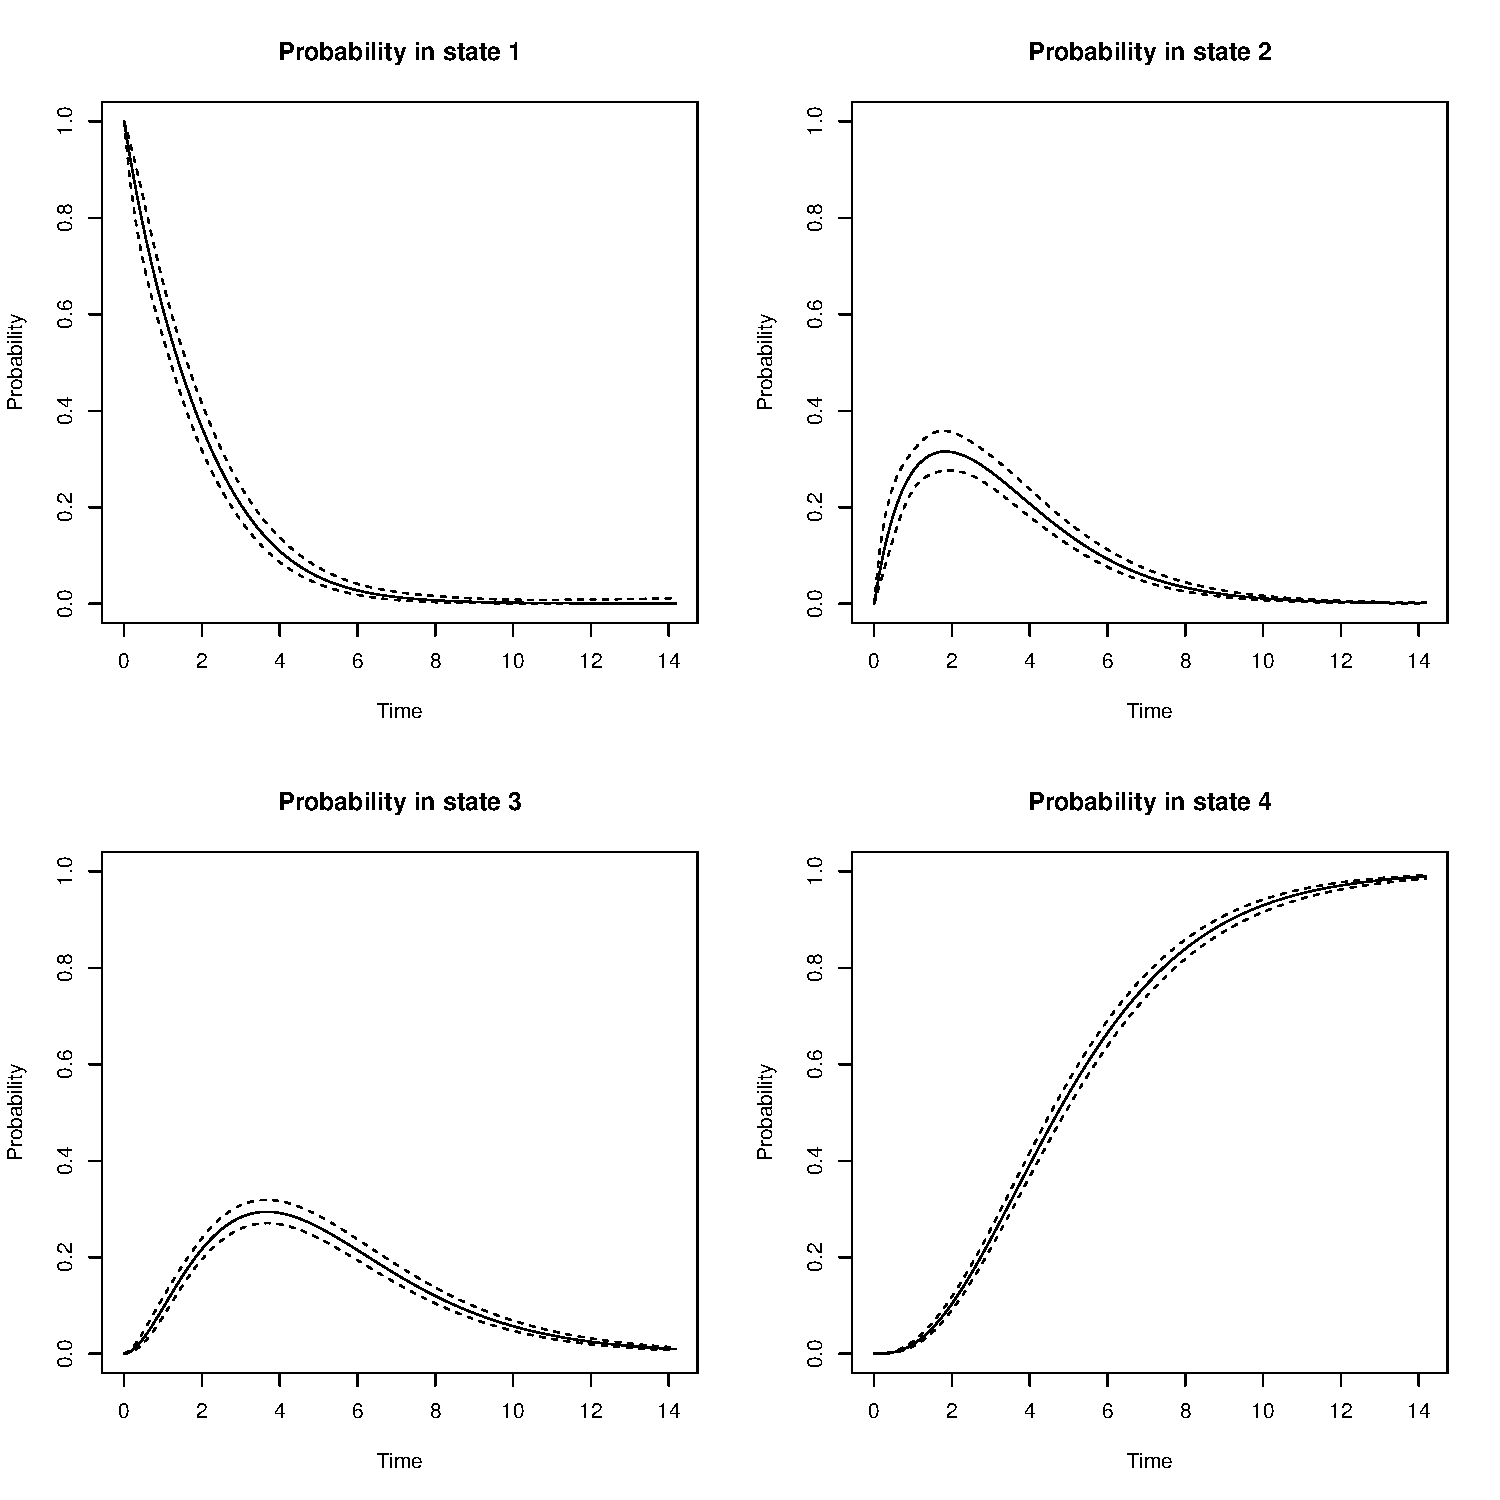
\includegraphics[scale=0.3]{Figures/bspline_fit1.pdf}
\end{center}
\end{figure}

However we can, for instance, produce a plot of the estimated transition intensities, for a subject with covariate values $(1,0)$ by using:

\begin{verbatim}
plot(bspline_fit, what="intensities", covvalue=c(1,0))
\end{verbatim}
\begin{figure}[ht]
\begin{center}
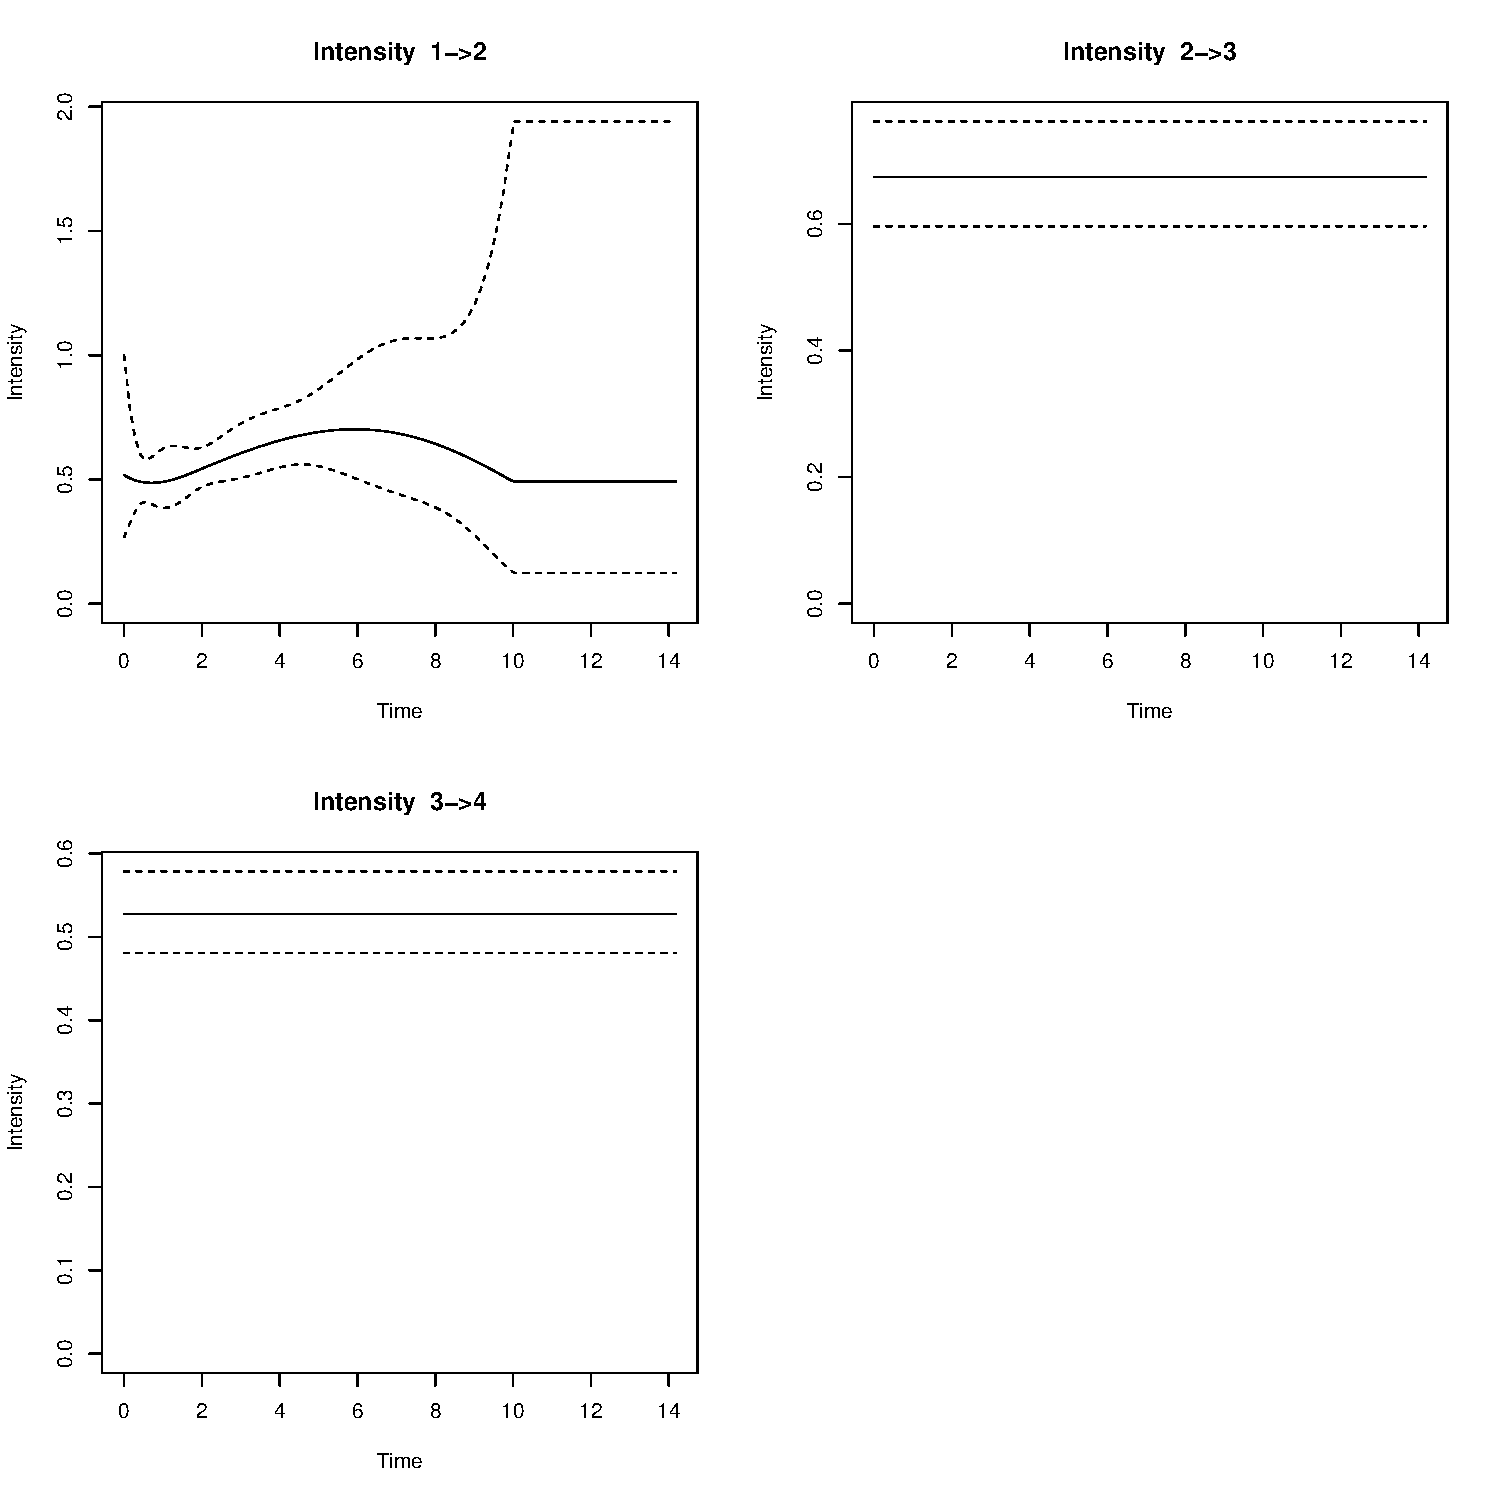
\includegraphics[scale=0.3]{Figures/bspline_fit2.pdf}
\end{center}
\end{figure}


There is apparently no obvious trend in the transition intensities, beyond some indication of an increased rate between 2 and 6 years.

Similarly, the estimated matrix of misclassification probabilities can be obtained using
\begin{verbatim}
ematrix.nhm(bspline_fit)
\end{verbatim}
\begin{verbout}
$emat
           [,1]       [,2]       [,3] [,4]
[1,] 0.91896279 0.08103721 0.00000000    0
[2,] 0.07046095 0.89906616 0.03047288    0
[3,] 0.00000000 0.09200885 0.90799115    0
[4,] 0.00000000 0.00000000 0.00000000    1

$SEemat
           [,1]       [,2]       [,3] [,4]
[1,] 0.02495268 0.02495268 0.00000000    0
[2,] 0.02408139 0.02511198 0.01740597    0
[3,] 0.00000000 0.01904015 0.01904015    0
[4,] 0.00000000 0.00000000 0.00000000    0
\end{verbout}

\section{Specifying bespoke models}

The \verb!bespoke! model type allows for user supplied functions for the generator matrix of intensities and its derivatives to be used with the package. There are two main motivations for supplying a bespoke function.
Firstly, it allows models not otherwise accommodated within the package to be fitted. These could include intensities from other parametric families than Gompertz or Weibull, or models with interactions between covariates and time.

The second motivation is to allow the computation time to be reduced for models that are accommodated within the existing functionality. The automatically created functions are slower than a specifically written function, particular for models which are sparse in the number of possible time or covariate effects.

\subsection{Example: Gompertz model}

Suppose firstly we wish to fit the same model as in [...]. The function needs to take \verb!t!, \verb!z! and \verb!x! as arguments, corresponding to the evaluation time, covariate vector and parameter vector, and should return a list elements \verb!q! - the intensities matrix and  \verb!qp! - the first derivatives of the intensities matrix.

\begin{verbatim}
fourstate_expgrowth<-function(t,z,x) {
  q12<-exp(x[1])
  q23<-exp(x[2])
  q34<-exp(x[3])
  i12<-q12*exp(x[4]*t + z[1]*x[7] + z[2]*x[8])
  i23<-q23*exp(x[5]*t)
  i34<-q34*exp(x[6]*t)
  q<-rbind(c(0,i12,0,0),c(0,0,i23,0),c(0,0,0,i34),c(0,0,0,0))
  diag(q) <- c(-i12,-i23,-i34,0)
  der<-array(0,c(4,4,8))
  der[1,1,1]<--i12
  der[1,2,1]<-i12
  der[2,2,2]<--i23
  der[2,3,2]<-i23
  der[3,3,3]<--i34
  der[3,4,3]<-i34
  der[,,4:6]<-t*der[,,1:3]
  der[1,1,7]<--i12*z[1]
  der[1,2,7]<-i12*z[1]
  der[1,1,8]<--i12*z[2]
  der[1,2,8]<-i12*z[2]
  Q<-list(q=q,qp=der)
  return(Q)
}
attr(fourstate_expgrowth,"npar")<-8
attr(fourstate_expgrowth,"parnames")<-c("1->2 base:","2->3 base:","3->4 base:","1->2 NH",
"2->3 NH","3->4 NH","Cov1","Cov2")
attr(fourstate_expgrowth,"parclass")<-c("Trans","Trans","Trans","Nonhom",
"Nonhom","Nonhom","Cov","Cov")
\end{verbatim}

The attributes are not essential, but will improve the informativeness of the output.

\begin{verbatim}
gomp_model_bespoke <- model.nhm(state~time, data=example_data1, subject = id, covariates=
  c("cov1","cov2"),   type="bespoke",trans=trans,intens=fourstate_expgrowth)
initpar <- c(model_msm$estimates,rep(0,5))
gomp_fit1b <- nhm(gomp_model_bespoke,initial=initpar)
\end{verbatim}
Exactly the same model as in \verb!gomp_fit1! is fitted, but the computation time in this case is around ..\% faster.

\subsection{Example: Gompertz model with interaction covariate effects}

Now we consider an extended version of the model, where the degree of time non-homogeneity depends on covariate 1. An extra parameter is added that introduces a common interaction between time and covariate 1 for the $1 \rightarrow 2$, $2 \rightarrow 3$ and $3 \rightarrow 4$ transitions. 

\begin{verbatim}
fourstate_expgrowth_int<-function(t,z,x) {
  q12<-exp(x[1])
  q23<-exp(x[2])
  q34<-exp(x[3])
  i12<-q12*exp((x[4]+z[1]*x[9])*t + z[1]*x[7] + z[2]*x[8])
  i23<-q23*exp((x[5]+z[1]*x[9])*t)
  i34<-q34*exp((x[6]+z[1]*x[9])*t)
  q<-rbind(c(0,i12,0,0),c(0,0,i23,0),c(0,0,0,i34),c(0,0,0,0))
  diag(q) <- c(-i12,-i23,-i34,0)
  der<-array(0,c(4,4,9))
  der[1,1,1]<--i12
  der[1,2,1]<-i12
  der[2,2,2]<--i23
  der[2,3,2]<-i23
  der[3,3,3]<--i34
  der[3,4,3]<-i34
  der[,,4:6]<-t*der[,,1:3]
  der[1,1,7]<--i12*z[1]
  der[1,2,7]<-i12*z[1]
  der[1,1,8]<--i12*z[2]
  der[1,2,8]<-i12*z[2]
  der[1,1,9]<--i12*z[1]*t
  der[1,2,9]<-i12*z[1]*t
  der[2,2,9]<--i23*z[1]*t
  der[2,3,9]<-i23*z[1]*t
  der[3,3,9]<--i34*z[1]*t
  der[3,4,9]<-i34*z[1]*t
  Q<-list(q=q,qp=der)
  return(Q)
}
attr(fourstate_expgrowth_int,"npar")<-9
attr(fourstate_expgrowth_int,"parnames")<-c("1->2 base:","2->3 base:","3->4 base:","1->2 NH",
"2->3 NH","3->4 NH","Cov1","Cov2","TimeEfCov1")
attr(fourstate_expgrowth_int,"parclass")<-c("Trans","Trans","Trans","Nonhom",
"Nonhom","Nonhom","Cov","Cov","Cov")
\end{verbatim}
Since this model is an extension of the previous one, it makes sense to use the estimates from the simpler model to obtain starting parameter estimates.

\begin{verbatim}
gomp_model_bespoke2 <- model.nhm(state~time, data=example_data1, subject = id, covariates=
  c("cov1","cov2"), type="bespoke",trans=trans,intens=fourstate_expgrowth_int)
initpar2 <- c(gomp_fit1b$par,0)
gomp_fit2 <- nhm(gomp_model_bespoke2,initial=initpar2)
gomp_fit2
\end{verbatim}
\begin{verbout}
               Est Low 95%  Up 95%
1->2 base: -0.9004 -1.0412 -0.7596
2->3 base: -0.3902 -0.5361 -0.2443
3->4 base: -0.6325 -0.8086 -0.4565
1->2 NH     0.0769  0.0294  0.1244
2->3 NH    -0.0086 -0.0473  0.0300
3->4 NH    -0.0096 -0.0459  0.0267
Cov1        0.4760  0.3293  0.6228
Cov2       -0.3179 -0.3899 -0.2458
TimeEfCov1  0.0077 -0.0149  0.0304

Deviance: 5789.49
\end{verbout}
In this case, the additional covariate does not improve the fit, which may be verified using \verb!anova!
\begin{verbatim}
anova(gomp_fit1b,gomp_fit2)
\end{verbatim}
\begin{verbout}
$LRS
[1] 0.4440297

$df
[1] 1

$p
[1] 0.5051839
\end{verbout}

\section{Left truncation}
\label{sec_left_trunc}

For multi-state data arising from cohort studies, the natural choice of time scale may be patient age, rather than time in the study. Moreover, the aim of the analysis may be to obtain an estimate of the target population's transition intensities as a function of age. However, patients will only be recruited into the study conditional on survival to their age at the calendar date the study began which we can denote as $t_{0i}$. Depending on the inclusion criteria or recruitment method, entry into the study may also be conditional on occupation of a specific state (or subset of the non-absorbing states). In general we can denote this set of states as $\mathcal{L}$ which should be a subset of $\{1,\ldots,R\}$.

For models without misclassification, if the state at a patient's entry age is known (either because it is fixed, e.g. state 1, or because their status is observed at entry) then it is not necessary to do anything except include (or, where necessary, impute) their state at entry in the supplied data. 

In contrast, if the state at $t_{0i}$ is not known or is subject to misclassification error, the left truncation needs to be accounted for in the likelihood. Specifically, we need to define a baseline age, $t_{00}$, where there is a fixed state occupation distribution (this could be all in state 1 with probability 1 or it can be defined via the initial state distribution options given in Section \ref{miscarg_sec}). The state occupation probability at $t_{0i}$ for a state $j \in \mathcal{L}$ is then given by
$$\pi_{ij}(t_{0i}) = P(X_i(t_{0i}) = j) = \frac{\sum_{k} \pi^{(0)}_{ik} P_{kj}(t_{00}, t_{0i})}{\sum_{l \in \mathcal{L}} \sum_{k} \pi^{(0)}_{ik} P_{kl}(t_{00}, t_{0i})}$$
while $\pi_{ij}(t_{0i}) = 0$ for $j \notin \mathcal{L}$.
Here, we make the assumption that patients are recruited as a representative sample of those within state $\mathcal{L}$ at time $t_{0i}$.

By default, $t_{0i}$ is ascertained from the patient time given in the data for the patient's first observation. However, some datasets may only include patients who had at least $m$ visits/observations. 

Since version 0.1.2, this form of left-truncation can be accommodated within the modelling provided the overall model is of misclassification type. As noted above, a model can be forced to be treated as misclassification type by supplying a emat argument that is an $R \times R$ matrix of zeroes. \verb!firstobs='misc'! must be specified, but this should not be a restriction since censoring codes can be used for other situations.

\subsubsection*{Left truncation options}
When specifying the model using \verb!model.nhm!, the relevant arguments are 
\begin{itemize}
\item \verb!ltruncation_states! which should be a vector corresponding to $\mathcal{L}$ (the set of states which a patient could occupy at time of recruitment into the model). 
\item \verb!ltruncation_time! which should be a scalar that specifies the baseline age $t_{00}$ and defaults to 0.
\item \verb!ltruncation_entry! which should be a positive integer indicating at which observation number the left truncation conditions should apply. By default this is 1, if it is $m$ then it is assumed that the patient has been recruited into the study conditional on $X(t_{0i}) \in \mathcal{L}$ where $t_{0i}$ is their age at their $m$th observation.
\end{itemize}

If the state occupation probabilities are calculated using \verb!state_occupation_probabilities.nhm! (or \verb!plot! using \verb!what='stateoccup'!) for a model with left truncation then the initial state occupation probabilities at time \verb!time0! will be calculated assuming the initial state probabilities held at \verb!ltruncation_time! and that only occupation within \verb!ltruncation_states! is possible at \verb!time0!. Note that it is also possible to supply a list \verb!ltruncation! containing \verb!ltruncation_states! and \verb!ltruncation_time! in order to estimate the state occupation probabilities that would arise under different sampling schemes.

\subsection{Additional options}
Version 0.1.2. includes additional developmental options to 
\begin{enumerate}
\item allow testing of the assumption of non-informative observation via targeted score tests (using the \verb!inform! option in \verb!model.nhm!)
\item allow semi-Markov and misclassification hidden semi-Markov models defined as aggregated Markov processes (using the \verb!phasemap! option). Currently this can only be applied to `bespoke' type models.
\item estimate the expected time spent in each state of a fitted model, using the \verb!state_life_expectancy! function, and to estimate the expected hitting time for a fitted progressive model using \verb!expected_hitting_time!.
\end{enumerate}
Further details of these features will be provided in the future.

%Is this too long to include.
%\subsection{Semi-Markov models}
%
%The Markov assumption for $X(t)$ is primarily a mathematical convenience and may not necessarily provide a good fit to the true underlying process. One of the simplest way in which the Markov assumption may be violated is through duration dependence in the transition intensities, i.e. where the transition intensities depend on the time since entry into the state $t^{*}$ as well as patient time $t$; $q_{rs}(t, t^{*} ; \mathbf{z})$. In general, semi-Markov processes for panel observation data have intractable likelihoods. The exception is the situation where the observable semi-Markov process can be expressed as an aggregated Markov process. In the time-homogeneous case this property was exploited by Titman and Sharples (2009) to produce semi-Markov models where the sojourn distributions have Coxian phase-type distributions. However, in principle, the same idea can be applied to non-homogeneous processes. Specifically, we define a Markov process, $X^{*}(t)$, on $R^{*} > R$ states. $X(t)$ is then defined via some mapping from $\{1,\ldots,R^{*}\}$ to $\{1,\ldots,R\}$, e.g. $X(t)= j if X^{*}(t) \in \mathcal{U}_j$ for $j=1,\ldots,R$ where $\mathcal{U}_1,\ldots, \mathcal{U}_R$ form a partition of $\{1,\ldots,R^{*}\}$.
%
%In practice, the above specification can very easily lead to models that are not identifiable. Following the experience in Titman and Sharples (2009), a potential approach would be to restrict $X(t)$ to correspond to at most two states of $X^{*}(t)$, e.g. $i_1$ and $i_2$. 

\begin{thebibliography}{unsrt}

\bibitem{bhhh} Berndt E, Hall B, Hall R, Hausman J. (1974). Estimation and Inference in Nonlinear Structural Models. {\it Annals of Economic and Social Measurement.} {\bf 3}. 653--665.

\bibitem{coxmiller} Cox DR, Miller HD (1965).{\it The Theory of Stochastic Processes.} Chapman and Hall, London.

\bibitem{stavola} de Stavola BL. (1988). Testing Departures from Time Homogeneity in Multistate Markov Processes. {\it Journal of the Royal Statistical Society: Series C (Applied Statistics)} {\bf 37}. 242--250.

\bibitem{gay} Gay D.M. (1990), Usage summary for selected optimization routines. Computing Science Technical Report 153, AT\&T Bell Laboratories, Murray Hill.

\bibitem{maxLik} Henningsen A, Toomet O. (2011). maxLik: A package for maximum likelihood estimation in R.  {\it Computational Statistics}, {\bf 26}. 443--458.


\bibitem{jackson} Jackson C.H. (2011). Multi-State Models for Panel Data: The msm Package for R. {\it Journal of Statistical Software}, {\bf 38}(8), 1--29. \url{http://www.jstatsoft.org/v38/i08/}.

\bibitem{jackson2003} Jackson C.H, Sharples L.D., Thompson S.G, Duffy S.W, Couto E. (2003) Multistate Markov models for disease progression with classification error. {\it Journal of the Royal Statistical Society Series D} {\bf 52}:193-209

\bibitem{kalbfleisch} Kalbfleisch J.D, Lawless J.F. (1985) The analysis of panel data under a Markov assumption. {\it Journal of the American Statistical Association} {\bf 80}:863-871.

\bibitem{lystig} Lystig TC., Hughes JP. (2002) Exact computation of the observed information matrix for hidden Markov models. {\it Journal of Computational and Graphical Statistics}, {\bf 11}, 678--689. 

\bibitem{mandel} Mandel M. (2013) Simulation-based confidence intervals for functions with complicated derivatives. {\it The American Statistician}, {\bf 67}. 76--81.

\bibitem{lsoda} Petzold, Linda R. (1983) Automatic Selection of Methods for Solving Stiff and Nonstiff Systems of Ordinary Differential Equations. {\it Siam Journal of Scientific and Statistical Computing}, {\bf 4}. 136--148.

\bibitem{deSolve} Soetaert K, Petzoldt T, Woodrow Setzer R. (2010) Solving differential equations in R: Package deSolve. {\it Journal of Statistical Software}, {\bf 33}. 1--25

\bibitem{titman} Titman A.C. (2011). Flexible Nonhomogeneous Markov Models for Panel Observed Data. {\it Biometrics}, {\bf 67}. 780--787.

\end{thebibliography}
\end{document}


